% Chapter 1

\chapter{Future upgrades} % Main chapter title

\label{Chapter7} % For referencing the chapter elsewhere, use \ref{Chapter1} 
\section{Two AOM}
The next step would be to design the two AOM system. The system of two AOM can be controlled for upper and lower beam by using two OFS system as shown in Fig.~\ref{fig:Adv_Tx_module_layout}. Our study has several limitation about modeling studies of the elastic deformation. However, in order to measure high frequency, we need to understand elastic deformation.
Current technology is not enough since difference of the upper beam and lower beam are ignore. The strength of this study are well studied to handle various sources of uncertainties. For example, understanding the extent to which Pcal affects the mirror motion will help us set realistic model for analysis. Therefore, it is necessary to develop the technologies for improving systematic error understanding dramatically.
\begin{figure}
\begin{center}
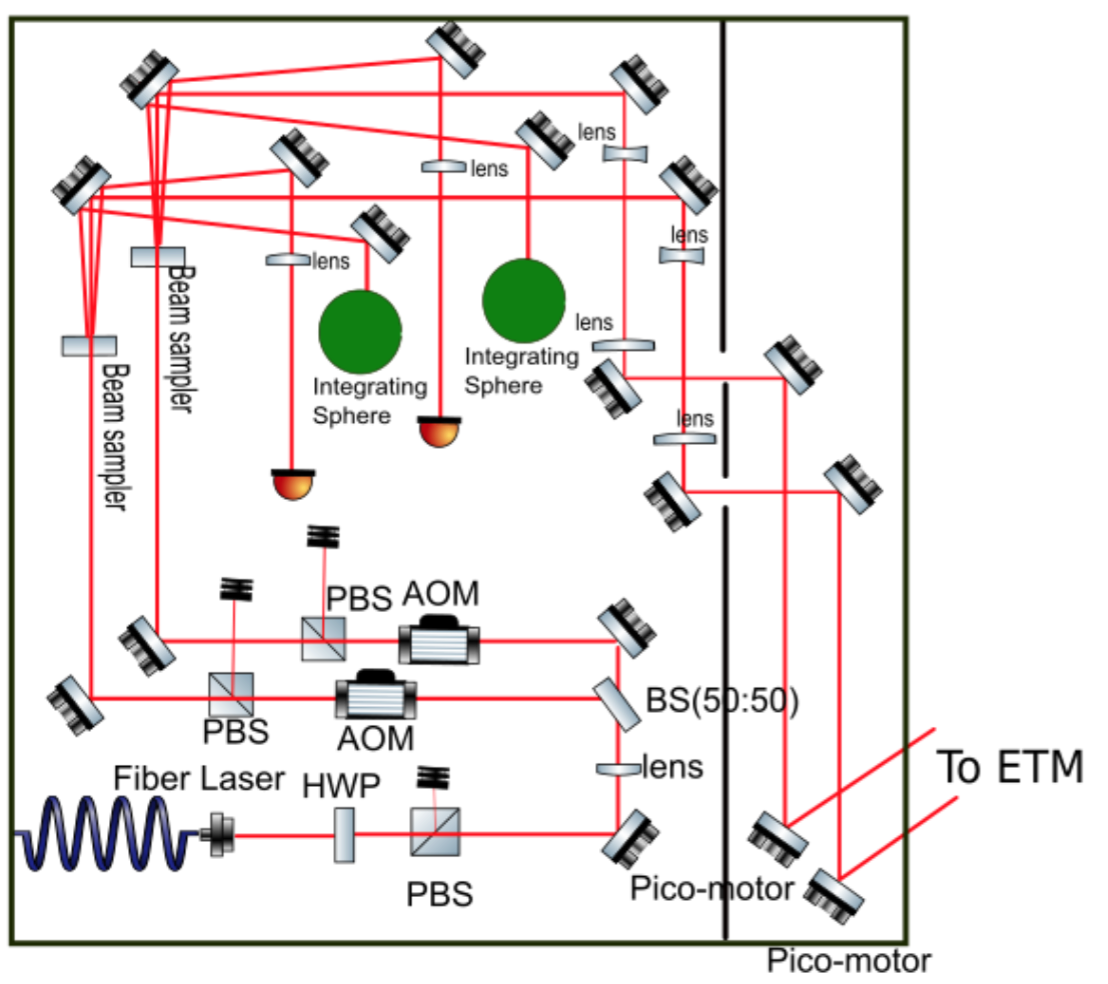
\includegraphics[width=14cm]{Figures/Adv_Tx_module_layout.eps}
\caption{Transmitter module with two AOM system.} 
\label{fig:Adv_Tx_module_layout} 
\end{center}
\end{figure}

\section{KAGRA Gold Standard}
Photo-detectors used in the transmitter and receiver modules to measure absolute laser power should be calibrated by laser power standard system. The Gold Standard of LIGO (GSL) is calibrated in NIST in US every year. A new test bench to calibrate LIGO PCAL photo-detectors were developed in NIST since LIGO PCAL uses unpopular wavelength laser of 1047nm to avoid to couple with main laser beam of interferometer with 1064nm in wavelength with keeping sufficient transmittance and reflectivity of optics. Finally, uncertainty of absolute laser power is mainly coming from uncertainty of the standard in NIST. 

In fact, absolute laser power is one of the worst precision items in the field of standard. Fig.~\ref{fig:Power_standard} shows performance comparison of laser power standard system in national standard institutions in the world, reported in 2009~\cite{EUROMET}. There is large inconsistency of about 4\% among the institutions. Rare cross-check of laser power standard among institutions carries out. In future work, we are planning to introduce new test bench of laser power standard with 1047nm in wavelength in AIST(National Institute of Advanced Industrial Science and Technology)  in Japan. We have already started discussion of such test bench development with a scientist in AIST. We newly make the Gold standard of KAGRA (GSK) using the integrating sphere with photo detector. By comparison with laser power standards both in NIST and AIST, and also with GSL and GSK themselves between aLIGO and KAGRA, we evaluate systematic errors of PCALs, and achieve to improve its accuracy. To calibrate the WSK, we plan to make a optical bench in Toyama university as shown in Fig.~\ref{fig:Toyama}. We will bring and compare the calibrated WSK and GSL in LHO.

\begin{figure}
\begin{center}
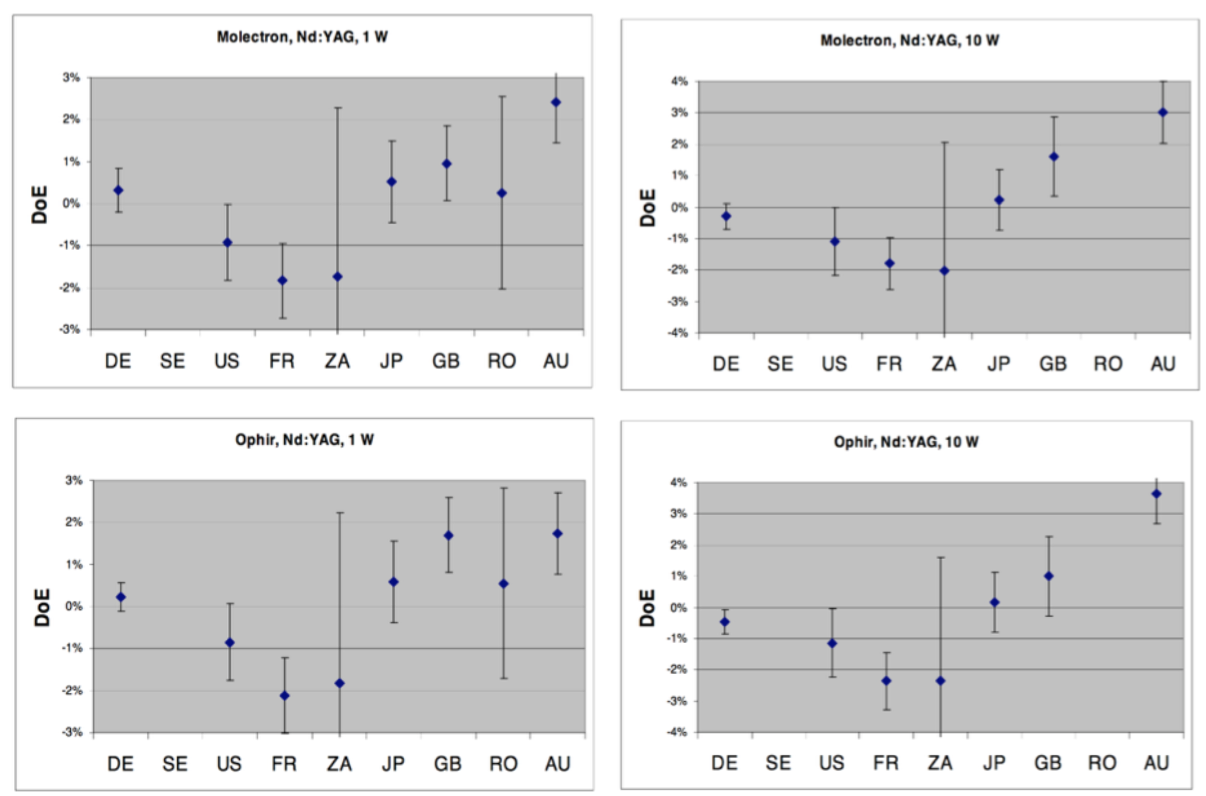
\includegraphics[width=14cm]{Figures/Power_standard.eps}
\caption{
Performance comparison of laser power standard system at 1064nm wavelength and 1W power in the national standard institutions in the world~\cite{EUROMET}.
} 
\label{fig:Power_standard} 
\end{center}
\end{figure}

\begin{figure}
\begin{center}
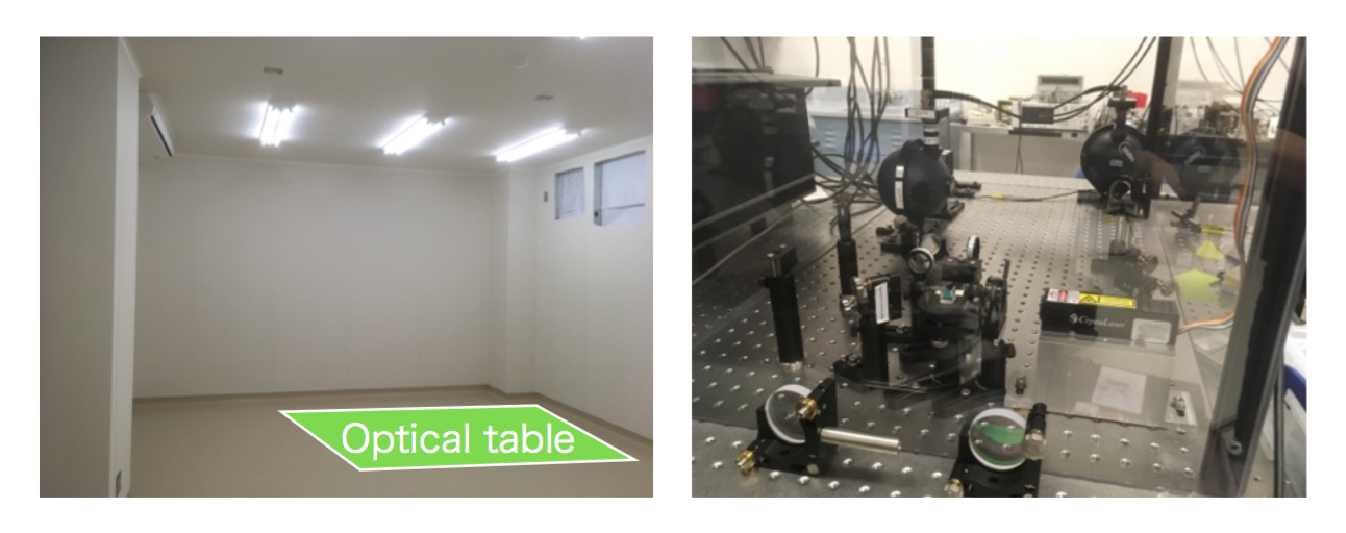
\includegraphics[width=14cm]{Figures/Toyama.eps}
\caption{.} 
\label{fig:Toyama} 
\end{center}
\end{figure}
